\documentclass[16pt,a4paper]{article}
\usepackage[top = 25.4mm, left=37mm, bottom=32mm, right=25.4mm]{geometry}
\usepackage{graphicx}
\usepackage{float}



\begin{document}

\tableofcontents

\clearpage
\pagebreak

\listoffigures

\pagebreak

\listoftables

\title{DESIGN AND DEVELOPMENT OF BROACHING FIXTURE FOR MACHINE PULLEY}
\maketitle
\linespread={1}
\parskip=1em

\paragraph{ABSTRACT\\}
Fixture plays an vital role in the manufacturing industry. Due to its wide application in the production plant the “Broaching fixture for machine pulley” has been designed and manufactured.  A systematic method was developed to generate a cutting strategy for the broach. The fixture is the necessary link between the part to be machined and the machine tool. Its design and implementation must be done efficiently in order to reduce the lead time to market the product. The fixture is particularly important because it is generally the deciding factor for the lead time and the quality of the operations. 
\\In machining fixtures, minimizing work piece deformation due to clamping and cutting forces is essential to maintain the machining accuracy. The various methodology used for clamping operation used in different application by various authors are reviewed. It is required in various industries according to their application. This can be achieved by selecting the optimal location of fixturing elements such as clamps. The fixture set up for component is done manually. For that more cycle time required for loading and unloading the material. So, there is need to develop system which can help in improving productivity and time. Fixtures reduce operation time and increases productivity and high quality of operation is possible.
\\ Due to the need of slot of dimension 6*2.8 in the machine pulley part the usage of fixture was inculcated due to which the pulley can be manufactured with accuracy, less human effort, reduced cyclic time and in mass quantity. “Shree Gajanan Industries” has the high demand of this pulley and it is periodically so that the fixture is to be used again. The fixture block should be mobile means it can be reused later when there is again need of same manufacturing plant. Later the force has to calculated on the fixture and the broaching tools nomenclature are studied and introduced.

\pagebreak

\section{INTRODUCTION}
The fixture is a special device for holding and maintaining a work piece in appropriate position during manufacturing operation. For supporting and clamping the work piece, this device is provided. Regular   checking, positioning, individual correcting and non-uniform quality in manufacturing process is terminated by fixture. This is used to reduce operation time and increase productivity. Fixture is widely used in the manufacturing industry for practical production because of its wide characteristics and functions. 
\\ To locate and position the work pieces for machining, inspection, assembly and other operations fixtures are used. A fixture consists of a set of locators and clamps. Locators are used to determine the position, setting the job and orientation of a work piece, whereas clamps apply clamping forces so that the work piece is pressed and set-up firmly against locators. Clamping has to be appropriately planned at the stage of machining fixture design. The design of a fixture is an highly complex and intuitive process, which require proper knowledge. Fixture design plays an important and vital role at the setup planning phase. Perfect fixture design is crucial for developing product quality in   different terms of accuracy, surface finish and precision of the machined parts In existing design the fixture set up is done manually, so the aim of this project is to replace with the traditional method to save time for loading and unloading of component. This mechanical fixture provides the manufacturer for flexibility in holding forces and to optimize design for machine operation as well as process functionability.
\\Successful fixture designs begin with a systematic and logical plan. With a complete analysis of the fixture's operational requirements, very few design problems in the designing may occur.  When they do, chances are some design requirements were underestimated or forgotten.The  work piece,  processing,  tooling  and  available  machine  tools  may  affect  the  extent  of  planning  needed. Preliminary analysis may take from a few hours up to several days for more complicated fixture designs.
\\ Fixtures are the tool used for locate and maintain the work piece in proper position during the manufacturing process. Fixtures are used to maintain and hold the parts firmly which are to be machined, it is used to produce the replica of the parts accurately. In order to produce the parts with required accuracy and dimensions the parts must be firmly and accurately fixed in to the fixtures. To obtain this, a fixture is designed and built to hold, support and locate the work piece to ensure that each and every work piece is machined within the specified limits which are mentioned in the part drawing. Tools like Set blocks, feeler or thickness gauges are used in the fixture to refer the work piece with the cutter tool. 
\\ A fixture should be securely fastened to the table of the machine upon which the work is to be done. Though largely used on milling machines, fixtures are also designed to hold the work for various operations on most of the standard machine tools. Fixtures vary in design based on the use of relatively simple tools to expensive or complicated devices. Fixture helps to simplify metalworking operations performed on special equipments. The fixture is a special tool for holding a work piece in proper position during manufacturing operation. For supporting and clamping the work piece, device is provided.
\\Frequent checking, positioning, individual marking and non-uniform quality in manufacturing process is eliminated by fixture. This increase productivity and reduce operation time. Fixture is widely used in the industry practical production because of feature and advantages. To locate and immobilize work pieces for machining, inspection, assembly and other operations fixtures are used. A fixture consists of a set of locators and clamps. Locators are used to determine the position and orientation of a work piece, whereas clamps exert clamping forces so that the work piece is pressed firmly against locators .Clamping has to be appropriately planned at the stage of machining fixture design.

\subsection{Problem Statement}
The manufactured part is the pulley which is to be design and analyzed. In which the specific notch was to be made has the pulley was to be manufactured in the mass quantity and there was increase demand for the workpiece repeatedly. So for that purpose the fixture was required which can help in for loading and unloading of the workpiece and increase the productivity by reducing the settling time of workpiece. Has the broaching machine been readily available so we according the specifications of the machine the fixture were required to be design. Before the design of the fixture when broaching operation was performed the excessive material was removed due to the misalignment of the tool or rapid movement of the broaching tool. Due to which the required dimensional notch was not obtained so to manufacture the 6*2.8 dimensional slot fixture was to be design accordingly. Fixture was to be design accordingly so that the tool can be perpendicular to the workpiece.
\\Along with that clamp should be also designed so that the fixture is maintained correctly or positioned on T-slot table of the broaching machine. So for that the force calculations is also required on the clamping device.

\subsection{Objective}
In manufacturing process, the time taken for changing of the job is important factor regarding efficiency of the work flow process. Thus the main aim or objective is to reduce the loading as well as unloading of the job which can increase the production rate .In broaching process there are extensive cutting process acting on the job and fixture as well. So the basic need of the fixture is to sustain the total amount of forces acting .Excessive use of machinery and due to cutting forces there might be chances of product to heat up which might affect the working purpose. Which in result might affect the geometric properties such as concentricity, parallelism. In such cases, with the help fixture we can maintain the properties by proper alignment and also provide path for coolant.

\subsection{Scope}
\begin{itemize}
\item The project plays very important role in an industry for increasing the productivity by decreasing the set-up time by decreasing the machine hour rate.
\item The broaching fixture is designed to reduce the cost of production as well as the elimination of setting up of tools the fixture will increase the production rate by providing more number of parts in less time.
\item By using number of locating pins for proper location, the accuracy of the fixture increased. Thus allows in improvement of the part to be broached.
\item The mass production is also achieved due to the fixture block and the tool is also guided.
\end{itemize}

\subsection{Methodology}

A method for designing a fixture comprising the steps of :
\begin{itemize}
\item The fixture is to be designed in such a way that it assists the broach cutter 
\item The tool should move in the guided direction
\item It should easily locate the workpiece with the help of 2 locator pins placed circumferentially
\item It should be easily changeable after the use for required product
\item The fixture should follow the 3-2-1 principle so that it will be fixed in x,y,z axis
\item Ease access to the operator for machining operation
\item For reducing the loading and unloading of the workpiece.
\item Effortless removal of the workpiece
\end{itemize}

A method for designing a broaching tool comprising the steps of :
\begin{itemize}
\item Providing geometry of a slot to be broached
\item Providing a material dependent initial minimum tooth rise for a broach tool that includes multiple broach inserts.
\item Calculating a number of broach inserts and teeth per insert based upon steps
\item Performing the broach inserts 
\item Calculating the stresses on the broach tool and deformation of the slot
\item Determining whether the slot dimensions are within desired specifications 
\item Revising the broach tool if the slot is outside the desired specifications, and performing the operation until the slot is within desired specifications 
\item Design characteristics of the broach tool resulting from performing 
\end{itemize}

\begin{figure}[h]
\centering
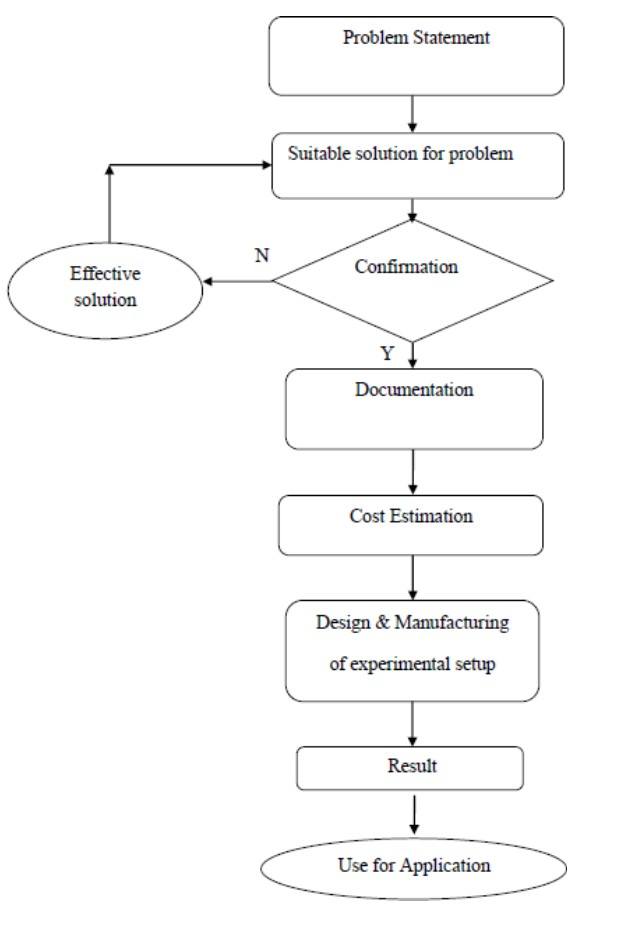
\includegraphics[scale=0.5]{methodology}
\caption{Flow Chart of Methodology}
\label{fig:methodology}
\end{figure}

\pagebreak

\section{LITERATURE REVIEW}

\begin{itemize}
\item Design and Analysis of Broach tool for Splines\\      
\\Broaching is the process of removing the metal with the help of broaching tool. The broaching tool has a tooth which are arranged in a row. Each tooth is successively higher than previous tooth and it removes more metal. Broaching is very efficient and rapid process. It has a wide range of application. In broaching process within a single pass both roughing and finishing can be done. It can produce both internal and external broach. With the help of broaching process, we can achieve better accuracy good productivity also a good surface finish. 
C language is use for development of program for design of broach tool  and to find various parameters such as pitch, length of tool and broaching force. Also sophisticated analysis 11 is used to analyze the stress developed in the cutting tools. 
\\Any error done in design of milling cutter or any other tool may result in rejection or it reduces life of tool, also there is decrease in its productivity. But if there is error in design of broaching tool results in tool breakage also rejection of parts.
\\The phase angle is equal to angle of a single point tool, it depends upon material to be cut. The back off an angle is providing relief to the tooth and it prevents excessive rubbing on a work. It reduces the friction between machine surface and the flanks of the tooth.
\\Broaching tools made up of material which is having high strength, hardness and toughness and also having good were resistance. It is mainly made up of high speed steel.\\     

\item Geometrical Optimization Of Broaching Tools By Levelling Of Cutting Forces\\  
\\Designing of broaching tool is very important step in broaching process, therefore designing of broaching tool we required various cutting forces and also cutting speed. In broaching process, we do machining of complicated parts without using a rotary motion.
This paper gives information about method in which we can minimize the length of Broach also increased tool life and quality by leveling the cutting forces. In broaching each tooth of broaching tool is designed. It has roughing teeth which takes first heavier cut, semi-finished teeth which follows roughing teeth and removes less amount of material and final finishing Teeth which perform finishing of operation. For analyzing cutting forces process monitoring is used. 
\\Process monitoring is a technique which used to find source of potential problem. In broaching it provides Information about various cutting forces acting on a tool on various section, also provide information about other machining parameter this all can be done with force measurement system. With the help of process monitoring of broaching tool we can improve tool design and part quality also eliminate various tooling problems.
\\With finite element method we can find stresses in a broaching tool. With two different rake angle we can measure tensile strength. This is done with analysis of broaching tool displacement at two different rake angles. In second step principal stresses where find out also finding of residual stresses on a broach. In order to reduce the tool and we can reduce the rock teeth on a broaching tool this can be done by milling of parts before broaching operation.\\    

\item A Flexible Fixture Design Method Research For Similar Automotive Body Parts Of Different Automobiles\\  
\\ Design method of a flexible fixture system for automotive body parts A modern automotive body has formed a mature structure hierarchy, which is usually made up of many parts welded together through dozens of procedures. Body in white of different automobiles usually contain a body frame, front and rear doors, a hood, a trunk lid, and left and right fenders. The body frame is usually composed of a front panel assembly, a rear panel assembly, left and right side panel assemblies, a roof assembly, and a floor assembly, and every assembly is also divided into sub-assemblies or parts until part levels. Although there are some differences in shape and structure for different automotive body parts, there is a lot of similarities on structures and dimensions for parts on the same position of different automobiles. Then, these similar parts of different automobiles are called as a product family in this article. Currently, new model replacements occur more and more quickly, in which the automotive body shape is usually one of the most changes. If a corresponding manufacturing system is set when a new automotive body is developed, the cost is greatly large. So, many automotive companies try to adopt flexible fixture systems to decrease development cost of a new automotive body. In this article, it supplies a flexible fixture design method for product families of automotive parts. This obtained fixture system can be used to locate and clamp similar parts of different automobiles during the welding process or measuring process. So, a lot of such equipment can be adopted to compose a complete welding line of an automotive body. This flexible welding line can be used to manufacture different automotive bodies through locating unite adjustments, which will greatly decrease manufacturing equipment cost and also save the production space.\\    

\item A Review On Design Of Fixtures\\
\\Steps of fixture design Successful fixture designs begin with a logical and systematic plan. With a complete analysis of the fixture's functional requirements, very few design problems occur. When they do, chances are some design requirements were forgotten or underestimated. The workpiece, processing, tooling and available machine tools may affect the extent of planning needed. Preliminary analysis may take from a few hours up to several days for more complicated fixture designs. Fixture design is a five step problem-solving process. The following is a detailed analysis of each step. Step 1: Define Requirements To initiate the fixture-design process, clearly state the problem to be solved or needs to be met. State these requirements as broadly as possible, but specifically enough to define the scope of the design project. The designer should ask some basic questions: Is the new tooling required for first-time production or to improve existing production? Step 2: Gather/Analyze Information Collect all relevant data and assemble it for evaluation. The main sources of information are the part print, the shop print is the current revision, and the processing information is up-to-date. Check with the design department for pending part revisions. An important part of the evaluation process is note taking. Complete, accurate notes allow designers to record important information. With these notes, they should be able to fill in all items on the "Checklist for Design Considerations." All ideas, thoughts, observations, and any other data about the part or fixture are then available for later reference. It is always better to have too many ideas about a particular design than too few. Four categories of design considerations need to be taken into account at this time: workpiece specifications, operation variables, availability of equipment, and personnel. These categories, while separately covered here, are actually interdependent. Each is an integral part of the evaluation phase and must be thoroughly thought out before beginning the fixture design. Step 3: Develop Several Options This phase of the fixture-design process requires the most creativity. A typical workpiece can be located and clamped several different ways. The natural tendency is to think of one solution, then develop and refine it while blocking out other, perhaps better solutions. A designer should brainstorm for several good tooling alternatives, not just choose one path right away. During this phase, the designer's goal should be adding options, not discarding them. In the interest of economy, alternative designs should be developed only far enough to make sure they are feasible and to do a cost estimate. 
\\The designer usually starts with at least three options: permanent, modular, and general-purpose work holding. Each of these options has many clamping and locating options of its own. The more standard locating and clamping devices that a designer is familiar with, the more creative he can be. Areas for locating a part include flat exterior surfaces (machined and unmachined), cylindrical and curved exterior surfaces. The exact procedure used to construct the preliminary design sketches is not as important as the items sketched. Generally, the preliminary sketch should start should start with the part to be fixtured. The required locating and supporting elements, including a base, should be the next items added. Then sketch the clamping devices. Finally, add the machine tool and cutting tools. Sketching these items together helps identify any problem areas in the design of the complete fixture. Step 4: Choose the Best Option The total cost to manufacture a part is the sum of per-piece run cost, setup cost, and tooling cost. Expressed as a formula: These variables are described below with sample values from three tooling options: a modular fixture, a permanent fixture, and a hydraulically powered permanent fixture. Step 5: Implement the Design The final phase of the fixture-design process consists of turning the chosen design approach into reality. Final details are decided, final drawings are made, and the tooling is built and tested. The following guidelines should be considered during the final-design process to make the fixture less costly while improving its efficiency. These rules are a mix of practical considerations, sound design practices, and common sense.\\    

\item Broaching Tool Degradation Characterization Based On Functional Descriptors\\     
\\ Proposed methodology approaches broach cutting edges are manufactured with relief angles on cutting edge flanks. This angle creates excessive noise in cutting edge images, which are difficult to compensate for, despite efforts to enhance the desirable contrast through lighting condition. To reduce this noise, the first task in the proposed method is to identify effective wear regions on each cutting edge at time 𝑡 by using adaptive image thresholding and process knowledge-based image filtering. Then, a linear function is fitted for the multiple cutting edges at each point in time, 𝑡, to describe the relationship between the wear area and the chip load. Finally, functional descriptors are used for unsupervised learning to determine degradation levels based on a k-means clustering scheme. \\    

\end{itemize}

\pagebreak

\section{DESIGN CONSIDERATION}
The points that are taken into consideration for designing a product are as following :


\begin{enumerate}
\item Fixture must be strong that the deflection in the fixture should be as less as possible and could withstand vibrations.
\item Another important design consideration is the clamping which should be fast enough and require less amount of effort.
\item They should also have the arrangement for easy removal  and there should also be provision for easy removal of chip.
\item It should always be preferred that there is maximum operation in a single setting of the workpiece. 
\item Base and body or frame with clamping features 
\item Locating elements for proper positioning and orientation of the blank 
\item Supporting surfaces and base 
\item Examine the work piece and finished component geometry and size.
\item Capacity and type of machine, its diversity in manufacturing.
\item Evaluation and performance ability of machines.
\item Rigidity of machining tool.
\item Level of accuracy required in the work and quality too.
\end{enumerate}

\subsection{Preliminary Design}

\begin{figure}[h]
\centering
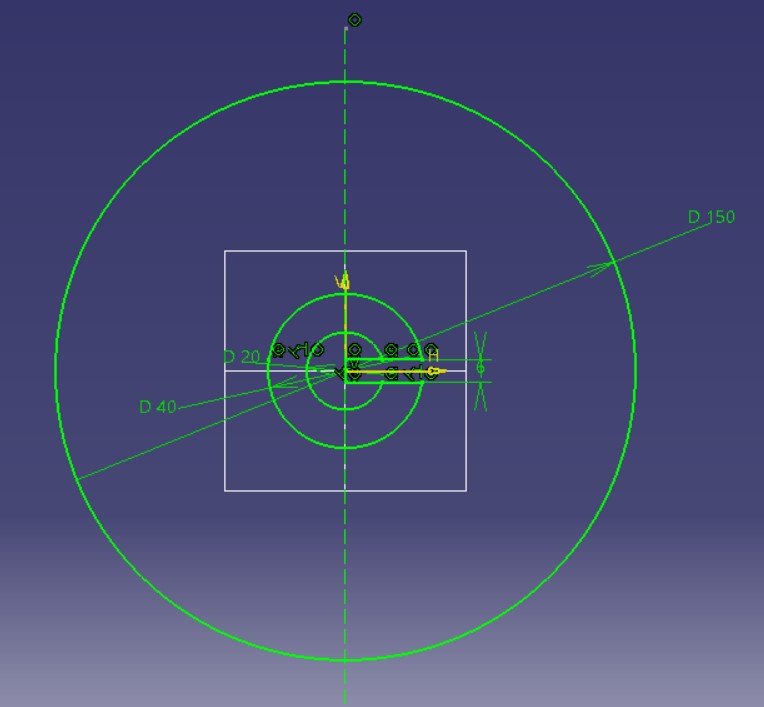
\includegraphics[scale=0.5]{Top View of Fixture}
\caption{Top View of Fixture Assembly in CATIA software}
\label{fig:TV of Fixture}
\end{figure}

The fixture is to be designed in such a way that it assists the broach cutter to move in guided direction and should easily locate the workpiece with the help of 2 locator pins placed circumferentially.
\\The fixture lets the operator easy access and effortless removal of the workpiece after the operation is completed.
\\The fixture is to be designed in such a way that it assists the broach cutter to move in guided direction and should easily locate the workpiece with the help of 2 locator pins placed circumferentially.
\\The pulley  is to be placed on the surface with the help of locator which also helps to maintain the accuracy .
\\The broach tool is to be cleaned by rubbing of the burr accumulated on within the teeth.

\subsection{Design of Fixture}
To meet all design criteria for work holder is impossible, compromise is inevitable. The most important hint of optimal design objectives is  positioning, holding and supporting functions that fixtures must fulfil.
\begin{enumerate}
\item Position: \\     
Fixture must above all else hold the work piece,  precisely in place to prevent 12 degrees of freedom, linear movement in the either direction about each axis.
\item Repeatability: \\   
Identical work piece specimens should be located by work holder in precisely the same space on repeated loading and unloading cycles. It should be impossible to hold the work piece incorrectly.
\item Adequate clamping forces: \\   
 The work holder must hold the work piece immobile against the forces of gravity. Centrifugal force, inertia force, wetting force, milling and the design must calculate these machines forces against the fixture holding capacity. The device must be rigid: clamping forces must be maintained.
\item Care during loading cycles:  \\    
As the work holders usually receive more punishment during the loading and unloading cycle  than during the machining operation. The device must endure impact and aberration for at least the  life of the job.

\end{enumerate}

Designing a fixture is a very complex task and it involves taking into consideration very minute details of manufacturing process. Even if a single detail is missed out then it may result in false design of fixture.
\\Broaching tool is a straight multi tooth cutter in which several cutting edges engage with the work piece simultaneously and each tooth removes a portion of material from the workpiece surface. Broaching cutter has a tapered flat or round profile with a series of teeth on its surface. Each successive tooth in a broaching tool is higher than the preceding one to perform the cutting action and remove material from the workpiece surface. Broaching tools in their general form can be geometrically divided into three main sections, namely, roughing, semi-finishing, and finishing. Roughing teeth remove the bulk of material from the workpiece, semi-finishing teeth produce the basic surface finish (surface quality), and finishing teeth provide the final surface finish and set geometrical and dimensional tolerances.
\\In broaching operation the broach tool slides in or out of the workpiece to convert the raw input material into finished product within just one stroke. The fixture should be designed in such a way that it should not block the path of the broach tool. Along with this the fixture should also help in proper alignment of the product aiding to lower cycle time.
\\The main function of the fixture is to hold the workpiece which is achieved by locking the various degrees of freedom of the fixture. To restrict the movement of the workpiece 3-2-1 location principle is used. To restrict complete movement of the product total 6 degrees of freedom are to be restricted which comprises of  rotary and linear 3 each.
\\Another Considerations in fixture design are specifications of the machine used. The fixture should also compensate for any  vibrations from the machine and should be designed for the maximum working force.\\    

Before moving towards any calculations we must firstly understand the tool geometry so as to calculate maximum force and then design the force accordingly :-

\begin{figure}[h]
\centering
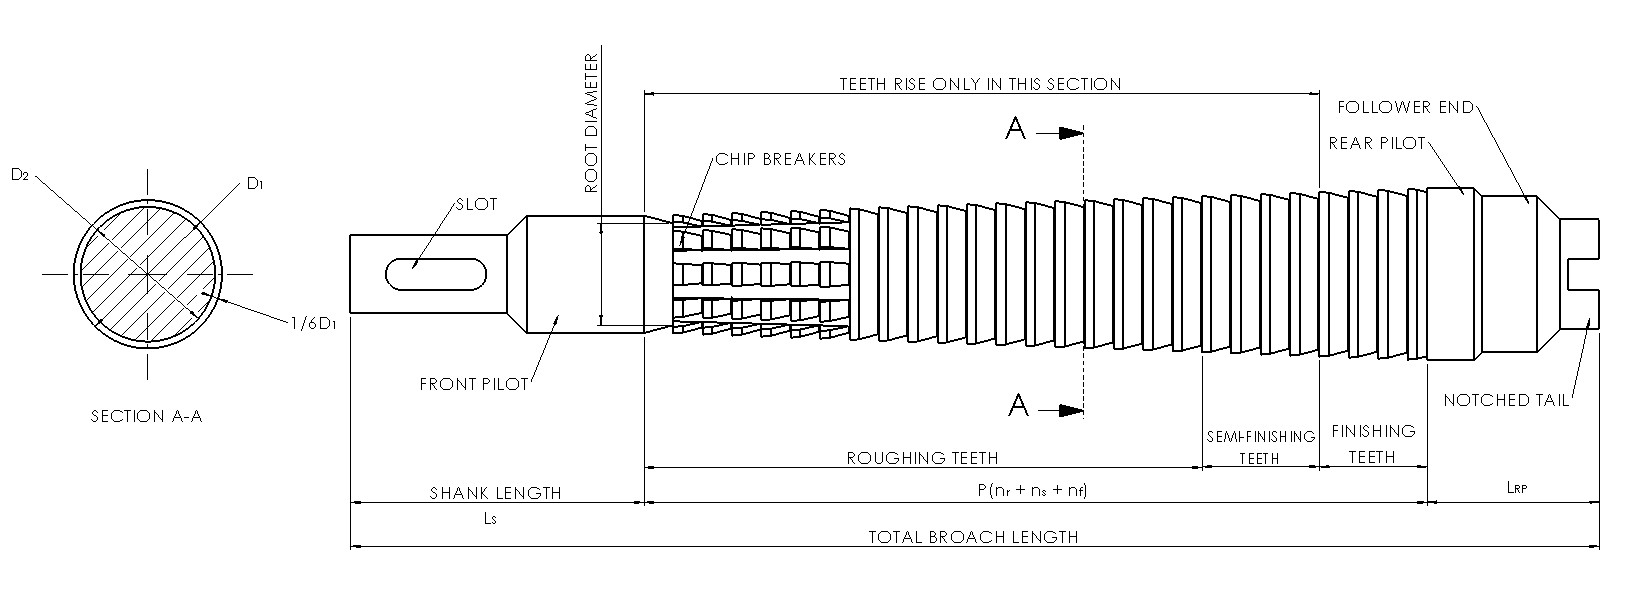
\includegraphics[scale=0.3]{Broach Tool Geometry}
\caption{Broach Tool Geometry}
\label{fig:Broach Tool Geometry}
\end{figure}

\begin{itemize}
\item Pull-Type Broach Tool :-
\begin{enumerate}
\item Pull End:- \\   
It is the handle of the pull broach tool which is used while pulling the broach tool.
\item Neck:- \\  
The neck connects the pull end to the root diameter.
\item Shank:- \\   
The part from the pull end to root diameter is a shank that is hold and pulled inside the machine. The length of the tool from pull end to root diameter is known as shank length.
\item Teeth:-  \\  
Teeth are placed in the pull-type broach tool after the shank. The size of the teeth increases progressively from start to end.
The teeth are divided into three portions in pull type broach tool.
\\These are:-

\begin{description}
\item [a] Cutting Teeth \\  
The portion of teeth near the shank is called cutting teeth. These teeth are also known as roughing teeth. The size of two consecutive teeth varies largely. The difference between their sizes is large. Cutting teeth will provide the maximum cut in the workpiece and remove maximum material from the workpiece as compared to other portions of teeth.
\item [b] Semi finishing teeth \\   
After cutting teeth, there are semi-finishing teeth. The difference between sizes of two teeth in semi finishing teeth is large but less than cutting teeth. Semi finishing teeth are used for semi finishing . These teeth remove very less material from the workpiece as compared to semi finishing teeth.
\item [c] Finishing Teeth \\   
The last portion of teeth after the semi finishing teeth are known as finishing teeth.These finishing teeth do not have variation in their sizes i.e all the finishing teeth are of nearly the same sizes.Finishing teeth will provide finishing to the cut produced by the cutting and semi finishing teeth. So these teeth are known as finishing teeth.
\end{description}

\item Rear Pilot :- \\   
After the finishing teeth, rear pilot is present in the pull type broach tool. It is used to balance the broach tool and keep it in alignment.
\item Follower End and Retriever :- \\     
They are present at end of the pull type broach tool. They both are supporting elements of the tool and supports the tool.

\end{enumerate}

\item Push Type Broach Tool. \\   
Push type broach tool is short in length than pull type broaching tool because it experiences compressive forces while it is pushed.It has fewer teeth than pull-type broach tool because chances of bending and getting broken is high as compressive forces are applied to it.
It provides a shorter cut than pull type broach.

\end{itemize}

The parts of the push type broach tool are the same as parts of pull type broach tool but the size of teeth and other parts of the broach tool is smaller than the tool of pull type broach. 

\begin{figure}[h]
\centering
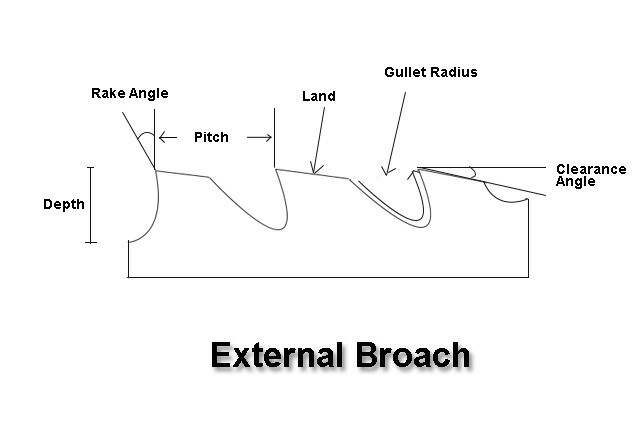
\includegraphics[scale=0.5]{Nomenclature of Broach Tool}
\caption{Nomenclature of Broach Tool}
\label{fig:Nomenclature of Broach Tool}
\end{figure}

\begin{description}

\item [a.] Land \\    
Land is present in the bottom of the teeth and it provides support to the cutting edge.
\item [b.] Rake \\   
Rake is provided in each tooth of the external broaching tool. The chip from the workpiece after the cutting process flow through this rake.
\item [c.] Clearance Angle \\  
Clearance Angle is the angle of the land or bottom part of the tool with the horizontal axis. It prevents friction between the teeth and workpiece and only the cutting edge of teeth is in contact with the workpiece while the cutting process.
\item [d.] Depth \\  
The height of each of the teeth is known as depth.
\item [e.] Pitch \\   
The distance between the cutting edges of any two teeth is known as pitch.
\item [f.] Gullet radius \\   
This radial space is present between two teeth through which the chip flow and go outside after getting curled.

\end{description}

\subsection{Calculations}

\begin{itemize}

\item In the case of broaching operation cutting speed V = speed at which the broach is pushed/pulled.
\item Apparent cutting edge engagement
\\ b = width of the broach  = 6 mm.
\item Actual cutting edge engagement
\\$ b_a$ = $\frac {b}{cos(\theta_s)}$ \\     \\   
$\theta_s$ = angle of inclination of the tooth w.r.t. the normal to the cutting velocity
\\= $\frac {6}{cos(15)}$ \\     
\\$b_a$=   6.211 mm
\item Apparent uncut chip thickness
\\ f = difference in heights of two consecutive teeth.
\\f = 0.05 mm
\item Effective or actual uncut chip thickness \\  
\\$f_a =  f cos (\theta_s)$\\    
\\ =  0.05*cos(15)\\   
\\$f_a$=  0.04827 mm
\item Area of uncut chip \\  
\\$f_b= 0.05 * 6 = 0.3 mm^2$
\item Metal removal rate/tooth = $ f_b.V$\\   
\\Metal removal rate/tooth $= 0.05 * 6 * 6 = 1.8 \frac {mm^3}{sec}$\\     
\item Machining time = $ \frac{(l_w + l_b)}{V}$          ($l_w$ = length of workpiece and $l_b$ = length of broach)   \\    
\\               = $ \frac {( 15 + 908)}{6}$\\   
\\ Machining time=153.833 sec

\end{itemize}

In broaching operation, only one motion, i.e. the primary cutting motion is provided by the machine (cutting speed is around  6 mm/sec). The feed motion is obtained by designing the teeth to be deeper progressively. (The cut per tooth is kept around 0.05 to 0.09 mm). Thus the shape of the broach determines the shape of the machined part.\\   

\begin{figure}[h]
\centering
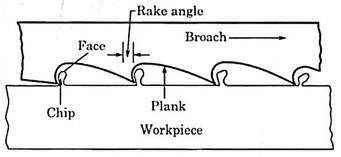
\includegraphics[scale=0.7]{External Broach}
\caption{External Broach}
\label{fig:External Broach}
\end{figure}

Cutting Force per Tooth = $\frac {w.S_s.cos(\lambda - \alpha)}{sin(\phi).cos(\phi + \lambda -\alpha)}$ Newtons \\  \\          
\\Where,
\\w = width of cut (In case of circular hole, w = circumference)
\\$\phi$ = shear angle = $90^0$
\\Co-efficient of friction =$\mu$ = 0.42 (between MS and EN-19)
\\$\lambda$ = Friction angle = $tan^{-1}(\mu)$ = $tan^{-1}$(0.42) = $22.78^0$
\\$\alpha$ = radial rake = $10^0$
\\f = cut per tooth = 0.05 mm
\\$S_s$ = ultimate shear stress of work material = 300 $N/mm^2$

Cutting Force per Tooth = $\frac {6 . 300 . cos (22.78 - 10)}{sin (90) . cos (90 + 22.78 - 10)}$ \\    \\    
\\Cutting Force per Tooth = 7935.55 N
\\Instanteneous broaching load = cutting force per tooth * number of teeth in contact 
\\                                                 = 7935.55 * 2 
\\Instanteneous broaching load =  15871.10 N   \\        
\\Now that as we have the Instanteneous broaching load on the job we can consider the line of action of force acting on the fixture through the workpiece. If we consider the fixture as a simply supported beam and the Instanteneous broaching load (W) to be point load acting on the centre of the beam then we are able to calculate the required clamping forces to hold the workpiece in position during the operation. 
\\The Instanteneous broaching load is calculated to be the maximum force that may be applied on the workpiece throughout the operation. Hence the values calculated for clamping forces will be more than enough to hold the workpiece. Assuming the fixture material to be Mild Steel having $S_{yt}$ = 465.97 N/$mm^2$

\begin{figure}[h]
\centering
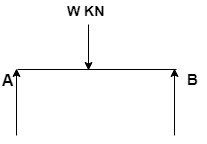
\includegraphics[scale=0.8]{Simply Supported Beam}
\caption{Free Body Diagram of fixture as simply supported beam carrying central point load}
\label{fig:Simply Supported Beam}
\end{figure}

Assuming equilibrium condition,           
$\sum F_x$ = 0, $\sum F_y$ = 0,$\sum M_A$  = 0 ; 
\\$R_A +  R_B$ = W
\\$R_A +  R_B$ = 15871.10 N \\    
\\$W*\frac {d}{2}$ - $R_B * d$ = 0
\\$R_B$ =$R_A$ = 7935.55 N
\\Therefore the clamping force is 7935.55 N.
\\The clamps are positioned in such a way that they grip the fixture by certain area. The diameter of the clamping area is 25 mm. As clamps are used to clamp the fixture on both sides the semicircular areas on either sides of the fixture combines to form a total circular area of 25 mm diameter.
\\The reaction forces cause certain compressive stress to develop in the fixture. We are going to analyse if the generated compressive stress is less than the permissible compressive stress of the fixture material. 
\\Compressive stress ($\sigma_c$)= Reaction Force / Resisting Area
\\Resisting Area = $\pi / 8$ * $25^2$ = 245.43 $mm^2$
\\Compressive stress ($\sigma_c$)= 7935.55 / 245.43 = 32.333 N/$mm^2$\\    
\\Permissible Compressive Stress ($\sigma_{cper}$) = $S_{yt}$ / 2
\\Permissible Compressive Stress ($\sigma_{cper}$) = 232.98 N/$mm^2$\\   
\\We can see that,
\\$\sigma_c$ < $\sigma_{cper}$\\    
\\Hence we know that our design is safe and we can use Mild Steel as a material for fixture.

\subsection{Part Modelling on CATIA}
CATIA is Computer Aided Three Dimensional Interactive Application used to model parts for various assemblies with ease and accuracy. We have used this software to generate models of different parts of our Fixture Assembly.

\begin{figure}[h]
\centering
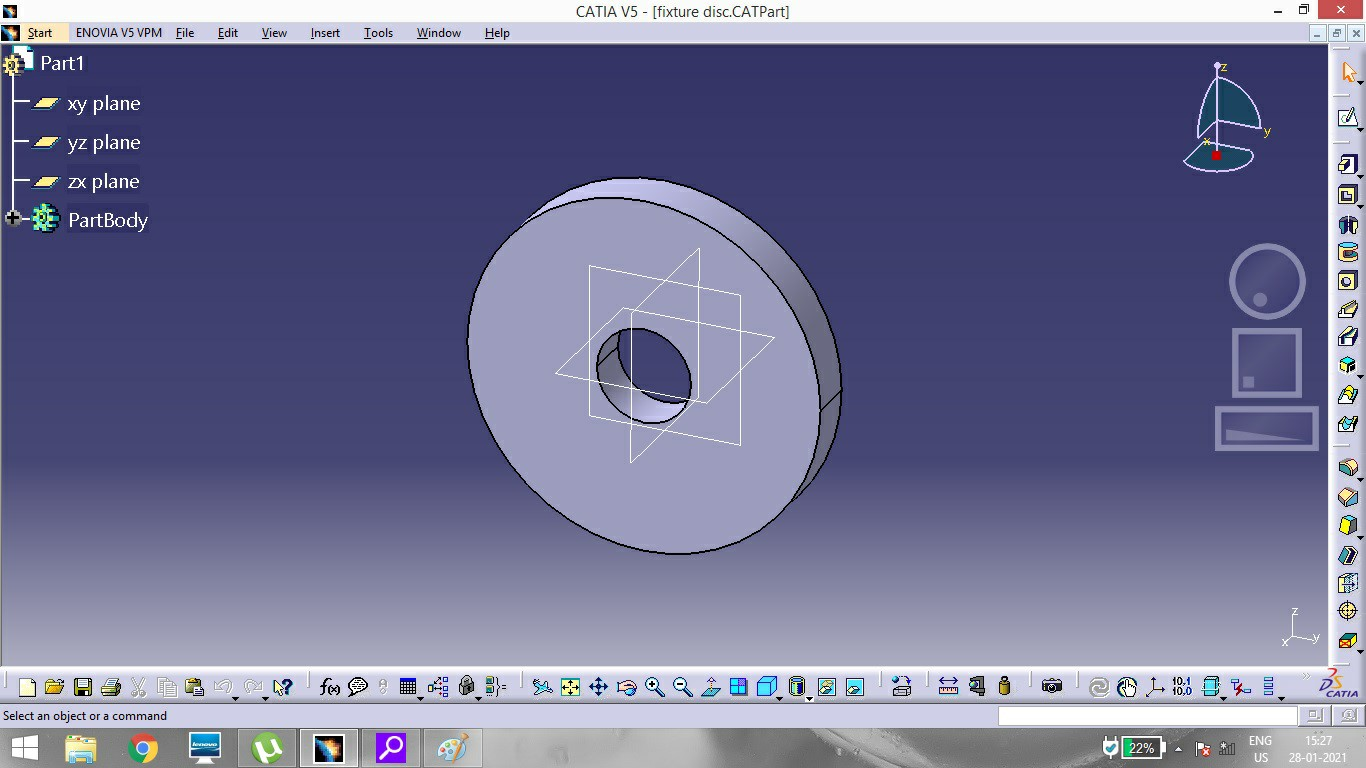
\includegraphics[scale=0.3]{Base Ring of Fixture}
\caption{Base Ring of Fixture}
\label{fig:Base Ring of Fixture}
\end{figure}

\begin{figure}[h]
\centering
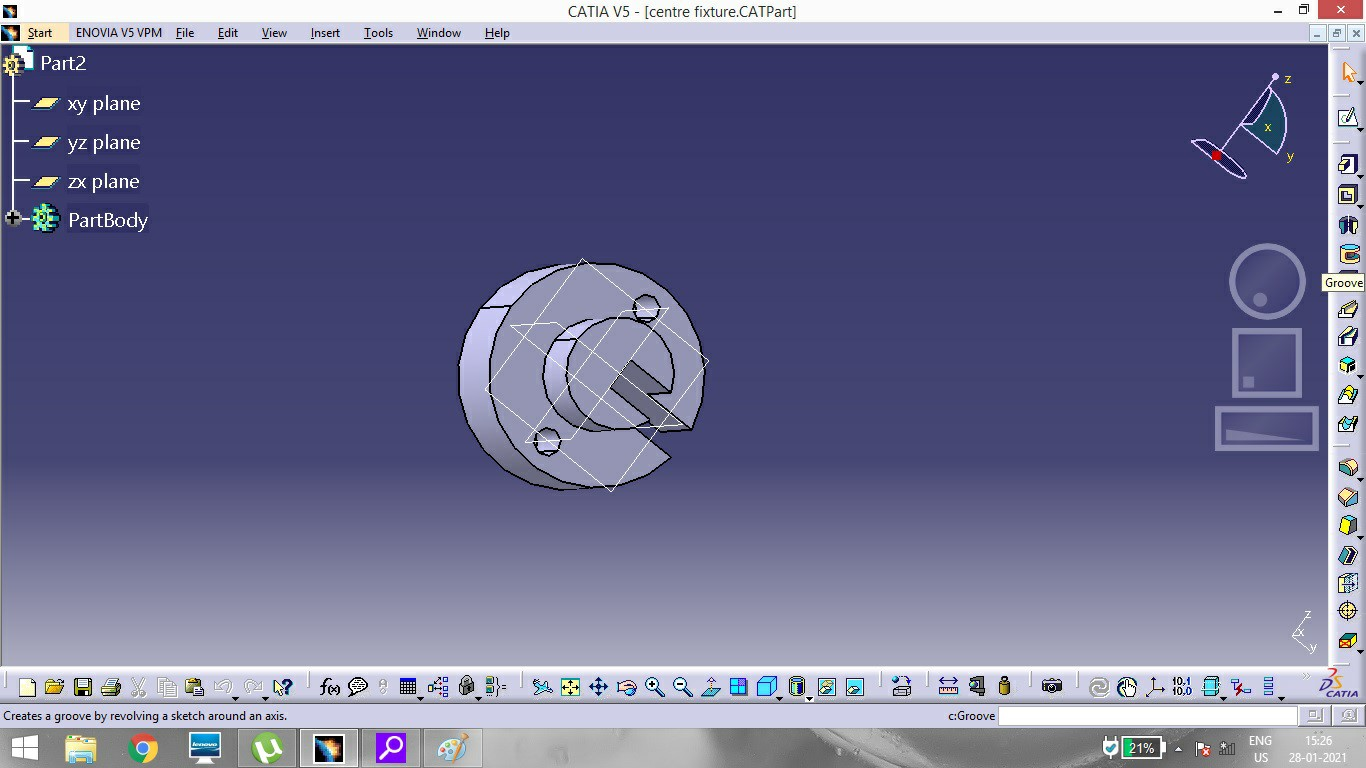
\includegraphics[scale=0.3]{Guide Ring of Fixture}
\caption{Guide Ring of Fixture}
\label{fig:Guide Ring of Fixture}
\end{figure}

\begin{figure}[H]
\centering
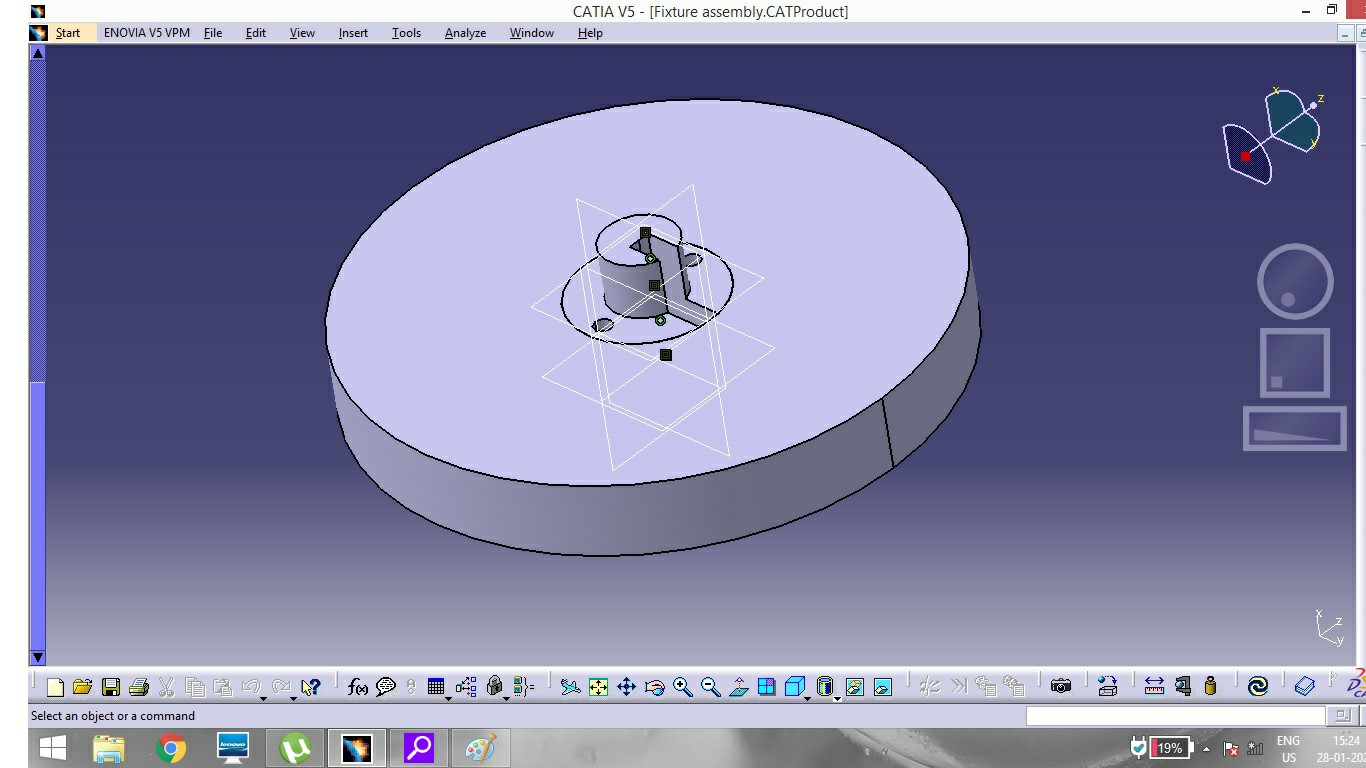
\includegraphics[scale=0.3]{Fixture Assembly}
\caption{Fixture Assembly}
\label{fig:Fixture Assembly}
\end{figure}

\subsection{Analysis of Forces on ANSYS Software}
ANSYS means Analysis System is software used to analyse various forces acting on the considered system. We used this software to Analyse and confirm the Analytically calculated forces of the system. Firstly we considered the fixture assembly model generated in CATIA and assumed it as simply supported beam by fixing its two ends. And considered the Instanteneous broaching load (W) to be acting centrally downwards. Now we analysed the compressive stress that was induced in the beam which was found to be within the range of permissible compressive stress $\sigma_{cper}$. This indicates that our analytical calculations being correct and precise.

\begin{figure}[H]
\centering
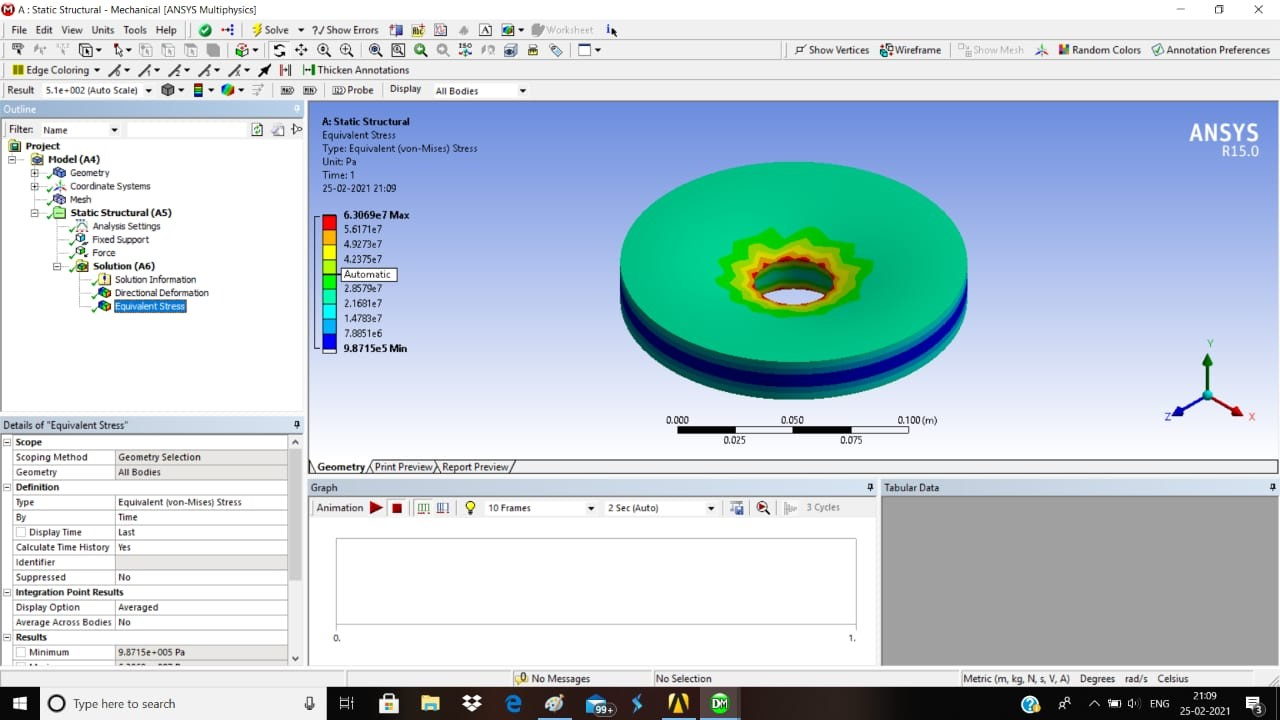
\includegraphics[scale=0.3]{Analysis on ANSYS Software}
\caption{Analysis on ANSYS Software}
\label{fig:Analysis on ANSYS Software}
\end{figure}

\pagebreak

\section{MATERIAL SELECTION}
Material selection is a step in the process of designing any physical object. In the context of product design, the main goal of material selection is to minimize cost while meeting product performance goals. Systematic selection of the best material for a given application begins with properties and costs of candidate materials. For example, a thermal blanket must have poor thermal conductivity in order to minimize heat transfer for a given temperature difference.
\\We have used two materials during our project,

\begin{enumerate}

\item EN 19 Steel :- 
\\EN 19 Steel is high quality alloy engineering steel. It has high tensile strength also having good ductility and shock resistance. The material leads itself well to any application where strength is primary consideration. It also offers good wear resistance. It is suitable for very high loading operation.

\begin{table}[H]

\centering
\caption{Grades and Standards of EN 19 in different countries}  
\begin{tabular}{| l | l | l |}
\hline
 Standard & Grades & Country \\
\hline
 EN 19 & BS 970-1955 & INDIA \\
\hline
 ASTM A29 & 4140 & USA \\
\hline
 DIN 17200 & 42CrMo & GERMAN \\
\hline
\end{tabular}

\end{table}

\begin{table}[H]

\centering
\caption{Composition of EN 19}
\begin{tabular}{| l | l |}
\hline
Element & Percentage \\
\hline
Carbon(C) & 0.45 \\
\hline
Silicon(Si) & 0.35 \\
\hline
Manganese(Mn) & 0.80 \\
\hline
Phosphorous(P) & 0.40 \\
\hline
Sulphur(S) & 0.40 \\
\hline
Chromium(Cr) & 1.4 \\
\hline
Molybdenum(Mo) & 0.40 \\
\hline
Iron(Fe) & Balance \\
\hline
\end{tabular}

\end{table}

\begin{table}[H]

\centering
\caption{Properties of EN 19}
\begin{tabular}{| l | l |}
\hline
Brinell Hardness(BHN) & 197 \\
\hline
Tensile Strength & 655 MPa \\
\hline
Yield Strength & 415 MPa \\
\hline
Elongation at break & 25.70 Percent \\
\hline
\end{tabular}

\end{table}


\item Mild Steel :- 
\\Mild Steel is most common steel used in industry. It has low amount of carbon. It is also known as low carbon steel. Due to its low carbon content, it is more malleable and suitable for welding. The less carbon in the steel, the more weldable and machinable it becomes. It has negligible amount of alloying elements which makes him more affordable as compare to other steels. Mild steel has high resistance to breakage also it has high tensile strength and impact strength. It cannot be herded through heat treatment process.
\\A small amount of carbon makes mild steel to change it properties. Different amount of carbon produces different types of steels. There are small spaces between the iron lattice. Carbon atoms get attached to this space and makes it stronger and harder. The harder the steel the lesser the ductility. Mild steel can be easily magnetized because of its ferromagnetic properties. So electrical devices can be made of mild steel.


\begin{table}[H]

\centering
\caption{Composition of Mild Steel}
\begin{tabular}{| l | l |}
\hline
Element & Percentage \\
\hline
Carbon(C) & 0.18 \\
\hline
Silicon(Si) & 0.40 \\
\hline
Manganese(Mn) & 0.80 \\
\hline
Phosphorous(P) & 0.040 \\
\hline
Sulphur(S) & 0.040 \\
\hline
Iron(Fe) & Balance \\
\hline
\end{tabular}

\end{table}

\begin{table}[H]

\centering
\caption{Properties of Mild Steel}
\begin{tabular}{| l | l |}
\hline
Brinell Hardness(BHN) & 130 \\
\hline
Tensile Strength & 495 MPa \\
\hline
Yield Strength & 465.97 MPa \\
\hline
Elongation at break & 15.0 Percent \\
\hline
\end{tabular}

\end{table}

\end{enumerate}

\pagebreak

\section{COST ESTIMATION OF PROJECT}

\begin{table}[H]

\centering
\caption{Cost Estimation of Project}
\begin{tabular}{| l | l | l |}
\hline
SR. No. &  Parameter & Costing \\
\hline
1 & Material & 2000 \\
\hline
2 & Machining & 600 \\
\hline
3 & Clamps & 1500 \\
\hline
4 & Total & 4100 \\
\hline
\end{tabular}

\end{table}

\pagebreak

\section{CONCLUSION}

In a modern manufacturing environment, organizations must be responsive to the requirements of the customers and their specific needs and to fluctuating global market demands. To maintain its competitiveness in market share, the manufacturing firms must manufacture with  minimum amount of waste. The main focus of this research is to reduce the setup time for the machining process performed on a high accuracy product, Machine Pulley.

\pagebreak

\section{REFERENCES}

\begin{itemize}
\item Shrikant.V. Peshatwar, L.P Raut “Design and development of Fixture for eccentric shaft: A Review” International Journal of Engineering Research and Applications.
\item https://www.engineeringenotes.com/metallurgy/broaching/broaching-parameters-and-characteristics-industries-metallurgy/22669
\item https://www.bing.com/search?q=press+clamp+pricesqs=nform=QBREsp=-1pq=press+clamp+pricessc=0-18sk=cvid=8B46E9D2839142308FA4B406FE8C81C7
\item https://www.bing.com/search?q=bright+hub+engineeringpc=COS2ptag=D052920-N0490A5AF4E3D53Cform=CONBDFconlogo=CT3335878SearchUrlPostfix=/searcht
\item https://www.sanfoundry.com/wp-content/uploads/2017/12/strength-materials-questions-answers-maximum-bending-moment-q9.png
\item https://civildigital.com/simply-supported-beam-with-point-load
\item www.engineersedge.com
\item Kuigang Yu1,2,3, Shiya Wang1 , Yanan Wang1,2,3 and Zhihong Yang1,2,3  2018, Vol. 10(2) 1–8  The Author(s) 2018 DOI: 10.1177/1687814018761272 “A flexible fixture design method research for similar automotive body parts of different automobiles.”
\item Malyadri Akula1 , K.Chandra Sekhar2 , Akula Nagendra3, E-ISSN 0976-3945 “DESIGN AND ANALYSIS OF BROACH TOOL FOR SPLINES.”
\item International Journal of Engineering Research and General Science Volume 2, Issue 2, Feb-Mar 2014 ISSN 2091-2730 Shailesh S.Pachbhai1 , Laukik P.Raut2 “A Review on Design of Fixtures.”
\end{itemize}





\end{document}